\documentclass[12pt]{article}

\usepackage[utf8]{inputenc}
\usepackage[brazil]{babel}
% \usepackage[english]{babel}

\usepackage{amsmath,amsthm,amsfonts,amssymb}
\usepackage{graphicx,cite,enumerate}
\usepackage{hyperref}
\usepackage{float}
\usepackage{booktabs}
\usepackage{multirow}
\usepackage[normalem]{ulem}
\useunder{\uline}{\ul}{}
\usepackage{booktabs}
\usepackage[table,xcdraw]{xcolor}
\usepackage{systeme}
\usepackage{array}
\usepackage{makecell}
\usepackage{afterpage}
\usepackage{algorithm} 
\usepackage{algpseudocode}
\usepackage{longtable}
\usepackage{adjustbox}
\usepackage{rotating}
\usepackage{quotes}
\usepackage{caption, subcaption}
\usepackage{etoolbox}

% My customization
%% Hide link boxes
\hypersetup{hidelinks}
%% Custom commands
% !TEX root = ../pmaluminum.tex


%%%%%%%%%%%%%%%%%%%
% My commands
%%%%%%%%%%%%%%%%%%%

\newcommand{\goal}[1]{[\textbf{Goal:} \blue{\emph{#1}}]}
\newcommand{\todo}[1]{[\textbf{TODO:} \cyan{\emph{#1}}]}
\newcommand{\question}[1]{[\emph{\textbf{Q:} \orange{#1}}]}
\newcommand{\todoeq}{[\green{\emph{EQ}}]}
\newcommand{\todofig}{[\green{\emph{FIG}}]}
% \newcommand{\source}[1]{[\green{\emph{src}#1}]}
\newcommand{\source}[1]{%
  \ifstrempty{#1}%
    {\green{[\emph{src}]}}%
    {\green{[\emph{#1} ]}}%
}


\newcommand{\diff}{\mathrm{d}}
\newcommand{\delScalar}[2]{\frac{\partial #1}{\partial #2}}
\newcommand{\delScalarSq}[2]{\frac{\partial^2 #1}{\partial #2^2}}
\newcommand{\delScalarTwo}[3]{\frac{\partial^2 #1}{\partial #2\partial #3}}
\newcommand{\delVector}[2]{\frac{\partial \mathbf{#1}}{\partial #2}}
\newcommand{\dScalar}[2]{\frac{\diff #1}{\diff #2}}
\newcommand{\dScalarSq}[2]{\frac{\diff^2 #1}{\diff #2^2}}
\newcommand{\dVector}[2]{\frac{\diff \mathbf{#1}}{\diff #2}}
\newcommand{\Nabla}{\boldsymbol{\nabla}}
\newcommand{\dr}[1]{\ \diff_{\mathrm{r}}\left(#1\right)}
\newcommand{\dt}[1]{\ \diff_{\mathrm{t}}\left(#1\right)}
% \newcommand{\dt}[1]{\dScalar{#1}{t}}

\newcommand{\cyan}[1]{\colorbox{cyan}{#1}}
\newcommand{\blue}[1]{\colorbox{blue}{#1}}
\newcommand{\red}[1]{\colorbox{red}{#1}}
\newcommand{\green}[1]{\colorbox{green}{#1}}
\newcommand{\yellow}[1]{\colorbox{yellow}{#1}}
\newcommand{\orange}[1]{\colorbox{orange}{#1}}

\newcommand{\Sh}{\mathrm{Sh}}
\newcommand{\Nu}{\mathrm{Nu}}
\newcommand{\Le}{\mathrm{Le}}
\newcommand{\Sc}{\mathrm{Sc}}
\newcommand{\Bi}{\mathrm{Bi}}
\newcommand{\Reynolds}{\mathrm{Re}}
\newcommand{\Prandtl}{\mathrm{Pr}}

\newcommand{\qAl}{\mathrm{Al}}
\newcommand{\qO}{\mathrm{O}}
\newcommand{\qH}{\mathrm{H}}
\newcommand{\qC}{\mathrm{C}}
\newcommand{\qN}{\mathrm{N}}
\newcommand{\qCO}{\mathrm{CO}}
\newcommand{\qAlAlOOO}{\qAl_2 \qO_3}
% \newcommand{\qH2O}{\H_2\O}
% \newcommand{\H}{\H_2}

\newcommand{\mrm}[1]{\mathrm{#1}}

\newcommand{\ejected}{\mrm{ejected}}
\newcommand{\const}{\mrm{const}}
\newcommand{\cond}{\mrm{cond}}
\newcommand{\conv}{\mrm{conv}}
\newcommand{\comb}{\mrm{comb}}
\newcommand{\melt}{\mrm{melt}}
\newcommand{\evap}{\mrm{evap}}
\newcommand{\boil}{\mrm{boil}}
\newcommand{\film}{\mrm{film}}
\newcommand{\rad}{\mrm{rad}}
\newcommand{\dep}{\mrm{dep}}
\newcommand{\net}{\mrm{net}}
\newcommand{\env}{\mrm{env}}
\newcommand{\flm}{\mrm{flm}}
\newcommand{\HSR}{\mrm{HSR}}
\newcommand{\HGR}{\mrm{HGR}}
\newcommand{\st}{\mrm{st}}

\newcommand{\qntdd}[2]{\ensuremath{#1 \, \mathrm{#2}}}

\renewcommand{\eqref}[1]{(\ref{#1})}

\newcommand{\from}[1]{
    \\
    \vspace{0.2cm} 
    {\small 
    \textbf{From}: \citeonline{#1}.
    }}

\newcommand{\fromme}{
    \\
    \vspace{0.2cm} 
    {\small 
    \textbf{From}: present author.
    }}
%% Line spacing
\usepackage{geometry}
\geometry{a4paper,portrait,hmargin={3cm,1.5cm}}
\renewcommand{\baselinestretch}{1.5}
%% Fonstize set at line 1


\title{\textbf{Multi-Scale Investigations For Reacting Multi-Phase Dispersed Spray Flows}}
\author{João Vinícius Hennings de Lara}
\date{April 2025}



\begin{document}

\maketitle
\newpage

\section{Introdução}


No cenario atual de busca pela transição energética e descarbonização, a pesquisa em combustão é mais importânte do que nunca.
Nesse contexto, os principais objetivos são reduzir emissões, adaptar os modelos para novos combustíveis mais limpos e para novos modos de combustão, necessários para motores mais limpos.

Análises históricas indicam que a transição para fontes de energia renováveis se dará ao longo de décadas \cite{MasriA2021}, [MASRI 1, 3 também]. Até lá, combustíveis fosseis mantém o seu domínio.
Além disso, no setor de transportes, a eletrificação dificilmente substituirá combustíveis fósseis em veículos de cargas pesadas ou para transporte aéreo ou marítmo, mesmo considerando previsões otimistas para o desevolvimento de baterias \cite{MasriA2021}. O mesmo pode ser dito para processos industriais intensivos em energia, como cimento e aço.

Uma opçao para a descarbonização desses setores é o uso de eletrocombustíveis, também chamados de \emph{e-fuels}, \emph{power-to-x} (PtX) ou \emph{powerfuels}.
Estes são combustíveis líquidos ou gasosos produzidos a partir de água, gas carbônico ($\text{CO}_2$), eventualmente nitrogênio $\text N_2$ e energias de fontes renováveis. 
Pode-se produzir, por exemplo: hidrogênio, metano, metanol, hidrocarbonetos líquidos (processo Fischer-Tropf), éteres de oximetileno (OMEs) e amônia (processo Haber-Bosch). source{MASRI 9}.
Os combustíveis PtX podem utilizar a infraestrutura de transporte, distribuição e armazenamento já existente dos combustíveis fósseis \source{MASRI 9-13} e podem chegar a ser neutros em termos de emissões, apesar que ainda mais caros que combustíveis de origem fóssil \source{MASRI 42, 43}. 

Outra alternativa para combustíveis de origem fóssil são os combustíveis verdes ou bio-combustíveis, produzidos a partir de platas. 
Por exemplo, o etanol e o metanol produzidos a partir do bagaço de cana, tecnologia desenvolvida no brasil; ou o etanol produzido a partir de milho, como nos estados Unidos; ou o metano advindo da biomassa. \source
Esses combustíveis reduzem  ...

Outra alternativa ainda é o uso de pós metálicos...

% A eletrólise da água produz hidrogênio, $\text H_2$.
% Hidrogênio com gas carbônico pode produzir hidrocarbonetos a partir do processo Fischer-Tropsch, ou metano, metanol ou éteres de oximetileno (OMEs).
% Por outro lado, hidrogênio também pode ser utilizado diretamente em células de combustível ou em motores de combustão futuros, ou produzir amônmia a partir do processo de Haber-Bosch.  



% Necessidade de trabalhar com combustão no contexto global.

% Necessidade de modelos HMT para partículas em simulações de combustão e sua importância


% Explain need for multicomponent modeling in current global context
% Explain need for modeling the interior of the droplet
% Explain need for droplet combustion model

% GAP: lack of models for single droplet combustion, modeling way behind pure evaporation
% GAP: lack of consistent multicomponent version of evaporation models and lack of multicomponent single-droplet burning models.
% GAP: lack of computationally affordable methods that account for droplet interior AND advanced evaporation/SDC models.

Exemplo de citação \cite{Wu2023}.





% \subsection{Motivação}
% \subsection{Lacunas}
% \subsection{Contribuição Científica}

\subsection{Objetivos}

Desenvolver um modelo     % Introdução Justificativa e síntese da bibliografia fundamental
% !TEX root = ../Proposta.tex


\section{Fundamentação Teórica}

% 2. Fundamentação Teórica (meio q Trabalhos preliminares)
%    1. Transferencia de calor e massa em gotículas (experiencia do grupo)
%       1. Multicomponente
%       2. Interior de gota
%    2. Single Droplet Burning (minha exp)
%       1. Monocomponente (contexto de sprays e meu trabalho)
%       2. Multicomponente (Sekularac e ArabkhalajA2024)
%       3. Probabilidade de acontecer
%    3. Turbulent spray combustion
%       1. Modelagem mecflu
%          1. LES, eqs de transporte, ATF
%       2. Modelagem da química
%          1. FGM


\subsection{Combustão Turbulenta de Sprays} \label{sec:teoria}

A combustão turbulenta de sprays é caracterizada pela competição de vários processos físicos e químicos, fortemente acoplados e em diferentes escalas de tempo e comprimento. 
Na formação de um spray turbulento, um jato de combustível líquido se quebra devido às instabiliades hidrodinâmicas de Kevin-Helmholz e Rayleigh-Taylor, formando gotas que se dispersam, deformam e atomizam devido às forças aerodinâmicas superando as tensões superficiais da gota \cite{JennyB2012}.
Isso forma o \textbf{regime denso} do spray, onde ocorrem também outros fenômenos como colisões, coalescência e interferência por esteira aerodinâmica, por turbulência ou por alteração da concentração de vapor de combustível devido à evaporação.
A medida que o jato se atomiza em gotas menores e dispersas, as gotas deixam de interferir umas nas outras e o regime é chamado de \textbf{disperso} ou \textbf{diluído}. 
Desde a sua formação, as gotas de combustível evaporam, fornecendo vapor combustível para a chama, que por sua vez influencia e é influenciada pelas próprias gotas e pela turbulência local.
Revisões detalhadas e com mais referências para processos e interações na combustão turbulenta de sprays podem ser encontradas em \cite{JennyB2012, MasriA2016, SanchezA2015, ZhouL2021,JiangX2010}.

O foco deste trabalho é na modelagem das escalas da gota (escala micro), que será utilizada em simulações CFD do spray e da chama (escala macro), considerando apenas a região diluida de um spray de combustível líquido.
Modelar a escala macro requer um modelo para a fase contínua, gasosa, um modelo para as reações químicas e um modelo para a fase dispersa, as gotas.
A modelagem da fase gasosa é discutida na Seção \ref{sec:gas} e um modelo, utilizado para simulações laminares reativas unidimensionais, é apresentado.
Duas abordagens para tratar a modelagem das reações químicas são discutidas na Seção \ref{sec:chem}.
As equações de evolução da gota são apresentadas na Seção \ref{sec:gotas} e os modelos de gota que preveem essa evolução são discutidos nas seções seguintes.
% \todo{Corregir esse link depois.}
% Dois exemplos de modelos para a fase contínua e para a química, escolhidos por relevância e experiência no grupo de pesquisa, serão apresentadas nas próximas Subseções \ref{sec:gas} e \ref{sec:chem}.
% Atenção especial será dada para a modelagem da gota, uma vez que o foco desse trabalho é desenvolver novos modelos para essa escala e investigar os efeitos na escala da chama.
% Modelos de transferência de calor e massa em gotas são discutidos nas Seções \ref{sec:MEC}. 

% Na abordagem macro, há duas fases nesse sistema: a fase contínua (gasosa) e a fase líquida (gotas); e ambas precisam de modelagem termo-física e química.
% Para a fase contínua, gasosa, isso se traduz nas equações de transporte, adequadas ao modelo de turbulência escolhido, e em uma modelagem química, que serão resolvidas durante a simulação.

% Já a fase contínua, por ser na escala da partícula, precisa ser modelada com um modelo analítico, já que a 

% Para a modelagem macro, a modelagem micro precisa ser incluida.
% Nas simulações Euler-Lagrange, foco deste trabalho e deste grupo de pesquisa,  

% A medida que as gotas se formam, elas evaporam, alterando a concentração
% A combustão turbulenta de sprays é um problema multi-fásico, multi-componente, multi-escala, multi-região e multi-físico. 

\subsubsection{Modelagem da Fase Contínua e Tratamento da Turbulência} \label{sec:gas}

As equações que governam a fase contínua são as equações de transporte de espécie, quantidade de movimento e energia, junto com as condições de contorno para a interface gás-líquido e relações termodinâmicas necessárias para o fechamento do problema.
Derivações desse conjunto de equações podem ser encontradas em livro-texto, por exemplo \cite{Williams1985,Kuo2005,Law2006,Glassman2008}.

Entretanto, utilizar essas equações dessa maneira requer resolver a interface das gotas, o que não é viável em simulações de chama de spray devido à diferença de escalas de comprimento entre as gotas e a chama e à quantidade de gotas em um spray (na ordem de grandeza de milhares a milhões).
Assim, uma abordagem para a simulação CFD de combustão de spray é representar as gotas como pontos infinitamente pequenos, cuja evolução no tempo e no espaço é acompanhada ao logo da simulação, a partir dos modelos de gota implementados.
Essa abordagem, de tratar a fase gasosa como contínua e as gotas como elementos pontuais no tempo e no espaço é chamada de \emph{Euler-Lagrange}.

A influência das gotas na fase contínua se dá, então, através de termos fonte, que inserem os efeitos do conjunto de gotas na célula em que elas estão inseridas, usando os modelos de gota. 
Essa abordagem é denominada PSIC - (\emph{Particle Source in Cell}) e a aproximação de uma partícula por um ponto é chamada de \emph{point particle approximation}.

Diferentes tratamentos matemáticos sobre as equações que descrevem a fase gasosa dão origem aos métodos DNS (\emph{Direct Numerical Simulation}), LES ( \emph{Large Eddy Simulation}) e RANS (\emph{Reynolds Averaged Navier-Stokes equations}). 
Cada um desses métodos aborda de maneira diferente a modelagem da turbulência e permite a simulação de escoamentos reativos turbulentos.

No que tange ao desenvolvimento de modelos para essas aplicações, é relevante testá-los em situações simplificadas, como em escoamentos reativos laminares primeiro.
O software unidimensional de escoamentos reativos CHEM1D \cite{Sommers1994PhD} é utilizado pelo grupo de pesquisa com esse propósito (por exemplo\cite{SacomanoF2018CTM,SacomanoF2019IJHMT,SacomanoF2021Fluids,SacomanoF2024CF,SacomanoF2025CF}).
Utilizando a formulação compressível para baixos números de Mach, as equações de conservação de massa, espécie e entalpia em uma dimensão 
\cite{SacomanoF2018CTM,SacomanoF2021Fluids,vanOijen2002CTM,vanOijen2016PECS}
são
\begin{equation}
    \frac{\diff \dot m}{\diff x} = \sum_k S_k,
\end{equation}
\begin{equation}
    \frac{\diff(\dot m Y_i)}{\diff x} -
    \frac{\diff}{\diff x} \left(
        \rho Y_i V_i
         %\frac{\lambda}{\mathrm{Le}_i c_p} \frac{\diff Y_i}{\diff x}
    \right) =
    \dot \omega_i + \delta_{ik} S_k,
\end{equation}
\begin{equation}
    \frac{\diff(\dot m h)}{\diff x}
    -
    \frac{\diff}{\diff x} 
        \left(
        \lambda %\frac{\lambda}{c_p} 
        \frac{\diff T}{\diff x} 
        \right)
    =
    \frac{\diff}{\diff x}
    \left[
        \rho \sum_{i=1}^N Y_i h_i V_i
        - R T \sum_{i=1}^N \frac{D_i^T}{X_i M_i}
        \frac{\diff X_i}{\diff x}
    \right]
    +
    S_h^L.
\end{equation}
Na primeira equação, $\dot m = \rho u$ é o fluxo de massa da mistura, $\rho$ a sua densidade e $u$ a sua velocidade na direção $x$, a coordenada espacial, e $S_k$ é o termo de acoplamento de massa entre fases da espécie $k$.
A segunda equação refere-se a espécie $i$: $Y_i$ é a fração mássica da espécie, $V_i$ a sua velocidade de difusão, $\dot \omega_i$ a sua taxa de produção/consumo e $\delta_{ik}$ o delta de Kronecker. 
A terceira equação é a da entalpia absoluta da mistura, $h$, em que $\lambda$ é a condutividade térmica da mistura, $T$ a sua temperatura. 
$h_i$ é a entalpia absoluta da espécie $i$, cuja fração mássica é $X_i$, massa molar $M_i$, e o coeficiente de difusão térmica $D_i^T$.
$S_h$ é o termo de acoplamento entre fases da entalpia.

Os termos de acoplamento de fases $S_k$ e $S_h$ são termos fonte de massa de vapor da espécie $k$ e de entalpia, respectivamente.
É através desses termos que os efeitos das gotas, calculados usando os modelos de gota, são inseridos na fase gasosa.
% Esses termos utilizam os modelos de gota, expostos nas Seções \ref{sec:MEC} e \ref{sec:MCGI}.

% a configuração de chama de propagação livre laminar em uma névoa de gotas foi simulada pelo grupo de pesquisa em \cite{SacomanoF2018CTM, SacomanoF2019IJHMT} no software CHEM1D \cite{Sommers1994PhD}.


\subsubsection{Modelagem Química} \label{sec:chem}

A modelagem química de maior fidelidade é chamada de química detalhada (DC - \emph{Detailed Chemistry}).
Essa abordagem utiliza um mecanismo químico com várias espécies e reações elementares, cada uma com uma taxa de reação modelada, por exemplo, por uma equação de Ahrrenius, para calcular as taxas de consumo ou produção das espécies principais e a formação de poluentes.
Os mecanismos podem ter dezenas de espécies e centenas de reações, o que torna esse método caro computacionalmente.

Uma alternativa para reduzir o custo computacional é o método FGM (\emph{Flamelet Generated Manifold}). 
Nesse método, a química detalhada é calculada previamente em vários cenários diferentes e uma biblioteca é construída, a qual conecta uma situação inicial, determinada por variáveis de controle, a uma situação final, pós combustão.
Tradicionalmente, duas variáveis de acesso são necessárias para determinar o espaço de variáveis (\emph{manifold}) do FGM, a fração de mistura %$Z=m_f/(m_f+m_{ox})$
e uma variável de progresso da reação \cite{PetersN2000}.
Em alguns trabalhos, como \cite{SacomanoF2018CTM}, a consideração de efeitos não adiabáticos força o uso da entalpia $h$ como uma terceira variável de acesso.
% usam três variáveis de controle, pois o efeito não adiabáticos  são considerados  na tabulação.
% Assim, além da fração de mistura $z$ e da váriável de progresso da reação $Y_{RPV}$,
% definida como uma combinação linear de $Y_{\text{CO}_2}$, $ Y_{\text H_2 \text O}$ e $ Y_{\text{CO}}$,
% % definida como $Y_{RPV}= Y_{\text{CO}_2} / {M_{\text{CO}_2}}+  Y_{\text H_2 \text O} / {2.5 M_{\text H_2 \text O}} + Y_{\text{CO}} / {1.5 M_{\text{CO}}}$,
% é utilizado também a entalpia $h$ como variável de acesso.
% As equações de transporte para as variáveis de controle tem a forma da equação abaixo, onde $\psi \in \lbrace z, Y_{RPV}, h\rbrace$ (\emph{cf.} \cite{SacomanoF2018CTM}).
% \begin{equation}
%     \frac{\partial \rho\psi}{\partial t} +
%     \frac{\partial \rho u \psi}{\partial s} =
%     \frac{\partial}{\partial s} \left(
%         \Gamma_\psi \frac{\partial \psi}{\partial s}
%         \right) +
%     \dot\omega_\psi +
%     S_h^L
% \end{equation} 

Outra estratégia para reduzir o custo computacional é o espessamento artificial de chama (ATF - \emph{Artificially Thickened Flame}), utilizada em simulações LES para reduzir o refino de malha necessário na frente de chama.
Essa metodologia foi desenvolvida em \cite{SacomanoF2017PhD} e aprimorada nos artigos seguintes \cite{SacomanoF2017CF, SacomanoF2020CF} para incluir o espessamento dinâmico, um efeito de interação chama-turbulência e a ampliação da taxa de evaporação de gotas atravessando a frente de chama.
% Em \cite{SacomanoF2017CF}, inclui-se o espessamento baseado nas propriedades da mistura e uma correção para a taxa de evaporação de gota durante atravessia da frente chama.
% Já em \cite{SacomanoF2020CF}, inclui-se o cálculo dinâmico de um termo para a interação chama turbulência.
% Nesses trabalhos, o tabelamento FGM é considerado adiabático e utiliza apenas duas vairáveis de controle: $z$ e $Y_{RPV}$.
% A equação de transporte dessas variáveis é modificada para o 
% espessamento da chama, tendo a forma dada pela equação abaixo, com $\psi \in \lbrace z, Y_{RPV}\rbrace$, (veja e.g. \cite{SacomanoF2017CF} para mais detalhes).
% \begin{equation}
%     \frac{\partial \bar \rho \widetilde \psi}{\partial t} + 
%     \frac{\partial \bar \rho \widetilde \psi \overline u_j}{\partial x_j} =
%     \frac{\partial }{\partial x_j} \left[ \left(
%     FE \frac{\bar\mu}{Sc_\psi} + (1-\Omega)\frac{\mu_t}{Sc_{t,\psi}}
%     \right) \frac{\partial \widetilde \psi}{\partial x_j}
%     \right] +
%     \frac{E}{F}\widetilde{\dot{\omega}_\psi} + 
%     \overline S_{\psi,\nu'}^{\text{Eul}}
% \end{equation}


\subsection{Resolução da Frente de Chama} \label{sec:FGM}



\subsubsection{Modelagem Da Fase Discreta} \label{sec:gotas}

A evolução das gotas na abordagem Euler-Lagrange com aproximação de gotas pontuais é regida por equações diferenciais ordinárias (EDOs) no tempo para a posição da gota, a sua massa e a sua entalpia ou temperatura.

Considere uma única gota dentro do spray, composta por $k=1,\ldots,n-1$ espécies (componentes).
O subscrito $d$ se refere à gota (\emph{droplet} em inglês).
Sua posição é dada pelo seu centro de massa $\mathbf X_d$, sua massa por $m_d = \sum_{i=1}^{n-1} m_{i}^k$ e sua temperatura, assumida uniforme em seu interior, por $T_d$.
A evolução da gota $k$ é então regida pelas EDOs \cite{JennyB2012}
\begin{equation}
    \frac{\diff^2 \mathbf X}{\diff t^2} =
    \frac{\mathbf f}{ m_{d,k}} -
    g \frac{\partial z}{\partial \mathbf x}
    \label{eq:Xd}
\end{equation}
\begin{equation}
    \frac{\diff m_{d}}{\diff t} = \sum_{k=1}^{n-1} \dot m_{d,k}
    \label{eq:md}
\end{equation}
\begin{equation}
    % \frac{\diff h^{k}_i}{\diff t} = \dot h^{k}_i
    m_d \sum_{k=1}^{n-1} Y_{L,k} c_{L,k} \frac{\diff T_d}{\diff t} = \dot q_d
    \label{eq:Td}
\end{equation}
em que $f$ representa as forças resultantes da fase gasosa na gota, $g$ é a constante da gravidade.
$\dot m_{d,k}$ é a taxa de variação de massa da espécie $k$ na gota e $\dot q_d$ o a taxa líquida de transferência de calor para a gota.
$ m_d \sum_k Y_{L,k} c_{L,k}$ é a capacidade térmica da gota, em que 
$Y_{L,k}$ e $C_{L,k}$ são a fração mássica e o calor específico da  espécie $i$ na fase líquida.
Os termos $\mathbf f$, $\dot m_{d,k}$ e $\dot q_d$ são termos de acoplamento entre as fases na escala da gota, ou seja, representam a interação entre as fases líquida e gasosa na interface da gota.
Enquanto o primeiro termo é geralmente substituído por uma expressão semi-empírica para o arrasto e o segundo por um termo de flutuação (\emph{vd.} \cite[p. 16]{JennyB2012}), os dois últimos precisam de um HMT. 
% \question{Usar $h$ e $\dot h^{k}_i$ ou $T$ e $ \dot Q_\net$?}

O modelo HMT pode descrever, por exemplo, a evaporação do combustível líquido e vapor de combustível, que é então queimado utilizando um dos modelos de química como DC ou FGM.
O mesmo modelo pode descrever também, a condensação de uma espécie de volta para a gota, como o próprio combustível ou a água, no caso de combustíveis hidrofílicos como os álcoois (e.g. metanol e etanol).
Nesse cenário, o modelo HMT é denominado de Modelo de Evaporação e Condensação (MEC).

O uso de um MEC junto de um modelo de combustão gasosa como DC ou FGM representa uma chama de spray no modo de combustão de grupo externa ou combustão externa com frente de chama, onde as gotas evaporam e fornecem vapor combustível para frente de chama, que não está acoplada a nenhuma gota individualmente.
Ao contrário, a chama pode estar circundando uma única gota, na chamada combustão de gota isolada.
O HMT que modela esse modo de combustão de spray é o MCGI.
% O HMT que considera uma frente de chama envolvendo a 
% Para modelar a combustão de gota isolada, é necessário um novo modelo HMT para a gota, que inclua essa frente de chama envolvente, denominado Modelo de Combustão de Gota Isolada (MCGI). 
% de acordo com a classificação de Chiu \source{Chiu1977, Chiu1982}
% Entretanto, não representa a combustão de gota isolada, já que, nesse cenário, a combustão ocorre na mesma escala que a gota.
% #TODO 1 revisar ligação aqui (ver review, parte roxa)


\subsection{Modelos de Evaporação e Condensação (MEC)} \label{sec:MEC}

% Desenvolver e testar esses modelos analíticos é o foco deste trabalho.

Na escala de uma gota, o problema pode ser dividido em duas regiões segregadas: a gota, líquida; e o gás ambiente circundante. 
Cada região é governada por um conjunto de equações.
Ambas regiões podem ser resolvidas numericamente (simuladas) ou representadas por um resultado analítico de um modelo, com diferentes graus de fidelidade.
Trabalhos que resolvem numericamente tanto o interior quanto o exterior da gota são capazes de simular muitos efeitos físicos a um elevado custo computacional. %(veja \source{Resolved evap small scale.}).
Em aplicações CFD, geralmente uma solução analítica é utilizada para a descrição espacial da fase gasosa, o que resulta nas taxas de trasnferência de calor massa para a gota, e as propriedades da gota são integradas no tempo.
Isso reduz o custo computacional e viabiliza o uso do modelo em simulações CFD na escala da chama de spray.

Essa separação é possível devido a hipótese de que a escala de tempo dos efeitos de transporte na região gasosa é muito mais rápida que a escala de tempo da mudança de temperatura da partícula.
Assim, efeitos transitórios na fase gasosa são desconsiderados e a evolução temporal da temperatura da partícula é desacoplada da transitóriedade da fase gasosa, que atinge estado permanente a cada instante da partícula.
Essa é a hipótese de regime quasi-estacionário.
Dessa forma, a fase gasosa pode ser resolvida analíticamente e a evolução da gota integrada no tempo.

% Para a região gasosa, é comum assumir que a escala de tempo dos efeitos de transporte nessa região é muito mais rápida que a escala de tempo da mudança de temperatura da partícula, ou seja, efeitos transitórios na fase gasosa não são considerados relevantes e o problema é quasi-estacionário.  

No que tange a região líquida, do interior da gota, geralmente assumida esférica, a hipótese mais simples é assumir uma distribuição homogênea de temperatura e espécie no interior da gota e negligenciar recirculação.
Isso elimina a necessidade de modelar o interior da gota.
Vale ressaltar que essas duas hipóteses, a de regime quasi-estacionário e a de interior de gota homogêneo, já foram utilizadas nas Equações \eqref{eq:md} e \eqref{eq:Td}.

Essa é a base para os modelos apresentados na Seção \ref{sec:RMM}.
Diferentes abordagem existem para considerar o interior da partícula; algumas são discutidas na Seção \ref{sec:int}.




\subsubsection{Modelos com Interior de Gota Homogêneo} \label{sec:RMM}

Naturalmente, os primeiros MECs a serem desenvolvidos consideravam gotas esféricas, \textbf{monocomponentes},com interior homogêneo, estacionárias em ambiente quiescente.
Nessa Seção, uma curta revisão dos MEC monocomponentes é apresentada, seguida pela apresentação do modelo multicomponente desenvolvido em \cite{SacomanoF2022IJHMT}.
A seção se encerra com alguns comentários sobre termodinâmica de mistura não ideal.
% Como os MECs multicomponente decaem para os MECs monocomponentes quando uma única espécie é utilizada, uma curta revisão histórica dos modelos monocomponentes é realizada, antes de apresentar um modelo multicomponente em detalhe.
% \todo{Melhorar essa merda.}

O primerio MEC foi desenvolvido por Fuchs \cite{Fuchs1959} na década de 1960 e é também chamado de modelo de Maxwell.
Esse modelo considera apenas e transporte por difusão e assume que temperatura da gota já está na sua temperatura equilíbrio de regime quasi-estacionário.
Assim, esse modelo não é capaz de representar o período de aquecimento da gota e gravemente subestima a taxa de variação de massa por considerar apenas o transporte por difusão.

A consideração do transporte por convecção em MECs, chamado de escoamento de Stefan (\emph{Stefan flow}), leva ao modelo de Stefan-Maxwell \cite{Law1978}.
A taxa de variação de massa da partícula nesse modelo pode ser dada tanto a partir do transporte de massa, quanto do transporte de energia, de usando os chamados número de transporte de Spalding.
Esse modelo também faz a hipótese de que a gota está na sua temperatura de equilíbrio no regime quasi-estacionário, não havendo modelo para o fluxo líquido de calor para a gota.

A hipótese de ambiente quiescente pode ser relaxada utilizando correlações experimentais para os números de Nusselt e de Sherwood, como as relações de Ranz-Marshall e Froessling \cite{Bird2002}. 
A adaptação dessas correlações para uma gota com escoamento de Stefan foi considerada no modelo de Abramzon-Sirignano \cite{Sirignano1989}, que também modelou o período de aquecimento da partícula, desfazendo-se da hipótese de temperatura de equilíbrio quasi-estacionária.

Uma hipótese realizada em todos os modelos supracitados é a de equilíbrio termodinâmico na interface líquido-vapor.
O relaxamento dessa hipótese deu origem ao modelo de Bellan-Harstad \cite{BellanJ1987}.
Ambos modelos de Abramzon-Sriginano e Bellan-Harstad foram combinados em uma única formulação matemática por Miller~et.~al em \cite{MillerR1998}.

Fugindo da metodologia da mecânica do contínuo, o modelo de Hertz-Knudsen-Langmuir \source{Langmuir} modela a taxa de variação da massa da gota baseada em cinética das partículas.

Os MECs \textbf{multicomponente} são naturalmente baseados nos MEC monocomponentes.
O modelo desenvolvido por Sacomano~et.~al em 2022 \cite{SacomanoF2022IJHMT} considera tanto a gota quanto os gases ambientes como multicomponentes, assim como a difusão diferencial das espécies e um comportamento de mistura não ideal.
% e a condição de não equilíbrio termodinâmico na interface líquido-vapor.
% e o modelo de Wang~et.~al \source{WangC2013CF} serão apresentados aqui.
Nesse modelo, a taxa de transferência de calor e de massa na interface da gota são dados por 
\begin{align}
    \dot q_d =& 4\pi R \lambda \frac{\Nu}{2}(T_\infty - T_s) + \sum_k \dot m_{d,k} L_k \label{eq:dmd} \\
    \dot m_d =& -4 \pi R \rho D_k \frac{\Sh_k}{2}B_{M,k} \label{eq:dqd}
\end{align}
em que $R$ é o raio da gota, $\lambda$ a condutividade térmica do gás ao redor da gota, $T_\infty$ a temperatura ambiente e $T_s$ a temperatura da superfície da gota. 
% O subscrito $d$ se refere à gota (\emph{droplet} em inglês) e $k$ à espécie, sendo $\dot m_{d,k}$ a taxa de variação de massa da espécie $k$ na gota 
$L_k$ é o calor latente de vaporização da espécie $k$.
$\rho$ é a densidade do gas circundante, $\Nu$ e $\Sh$ são os número de Nusselt e Sherwood, respectivamente, $D_k$ é o coeficiente de difusão multicomponente da espécie $k$ e $B_{M,k}$ é o número de transferência de Spalding de massa para a espécie $k$.
Os números de transferência de Spalding de energia e de massa nesse cenário são dados por
\begin{align}
    B_T =& \frac
        {(T_\infty - T_s) \sum_k c_{p,k}\dot m_{d,k}}
        {\dot q_d - \sum_k \dot m_{d,k} L_k} \label{eq:B_T}\\
    B_{M,k} =& \frac
        {\dot m_d Y_{k,s} - \dot m_d Y_{k,\infty}}
        {\dot m_{d,k} - \dot m_d Y_{k,s}}\label{eq:B_Mk}
\end{align}
onde, novamente os subíndices $s$ e $\infty$ se referem à superfície da gota e ao ambiente, $Y$ refere-se à fração mássica e, agora, $c_{p,k}$ refere-se ao calor específico a pressão constate da espécie $k$ na fase gasosa.
Nas equações \eqref{eq:dmd} e \eqref{eq:dqd}, os números de Nusselt e Sherwood podem ser utilizados para representar os efeitos de ambientes convectivos.
Porém, o fluxo de Stefan altera a troca de calor e massa da partícula, de modo que as correlações experimentais para gotas não evaporantes precisam ser adaptadas, como mostraram Abramzon e Sirignano \cite{Sirignano1989}.
A correção para utilizar as correlações empíricas para esses adimensionais  (\emph{c.f.} \cite[eqs. (8) e (9)]{SacomanoF2025CF}), representadas aqui nos símbolos $\Nu^0$ e $\Sh^0$, são
\begin{align}
    \Nu =& \frac{\ln \left|B_T + 1\right|}{B_T} \\
    \Sh =& \frac{\ln \left|B_{M,k} + 1\right|}{B_{M,k}}.
\end{align}

No cálculo de $B_{M,k}$, é necessário conhecer a fração mássica do vapor da espécie $k$ na superfície da gota.
Para misturas ideais, isso é feito pela Lei de Raoult, que dita $X_{k,s}=P^v_{k,s}/P_s$, onde $P^v_{k,s}$ é a pressão de vapor e $X_{k,s}$ é a fração molar de vapor da espécie $k$, relacionada a fração mássica pelas massas molares dos componentes da mistura gasosa \cite{Peters2010}.
A pressão de vapor pode ser obtida pela equação de Clapeyron, pela equação de Wagner ou pela equação de Antoine.
Uma comparação dos diferentes modelos para a pressão de vapor foi realizado por \cite{SacomanoF2019IJHMT}.

% O aspecto \textbf{não ideal da mistura} se manifesta em um desvio da Lei de Raoult, usada para calcular a fração molar de vapor de uma espécie a partir da pressão de vapor dessa espécie e da pressão total, todas na superfície da gota. 
Já em uma \textbf{mistura não ideal}, há um desvio da Lei de Raoult. 
A fração molar de vapor deve ser calculada por uma equação de estado não ideal ou através do cálculo dos coeficientes de atividade de cada espécie, o que representa a sua fugacidade \cite{Bird2002}.
Sacomano\etal{} em \cite{SacomanoF2022IJHMT} utilzaram os métodos de  Raoult (ideal) e UNIFAC (não-ideal) para calcular os coeficientes de fugacidade, enquanto Sacomano\etal{} em \cite{SacomanoF2025CF} utilizaram o método de van Laar.
Zanutto\etal{} \cite{ZanuttoC2019} utilizaram o método UNIFAC para os coeficientes de atividade da fase líquida e a equação de estado real Virial para a fase gasosa.
% Os trabalho de Sacomano\etal utilizam utilizam a abordagem de representar a fugacidade de cada espécie em termos dos seus coefientes de atividade . Em \cite{SacomanoF2022IJHMT}, os coeficientes de atividade 

% #TODO 5 mencionar que outro trabalho multicomponente rigoroso é ToniniS2015 ???

\subsubsection{Modelos para o Interor da Gota} \label{sec:int}

Em todos os modelos apresentados até agora, a temperatura e composição do interior da gota foram considerados ou (1) uniforme e contante (modelos que não representam o período de aquecimento da gota); (2) uniforme e variando no tempo (modelos com condutividade térmica e difusividade mássica da fase líquida infinitas).
Esses são os dois primeiros graus de complexidade da representação do interior da gota.
Os próximos são: (3) modelos com difusividade térmica e mássica finitas, mas sem recirculação; (4) modelos que consideram a recirculação em um fator de correção para as diffusividades térmica e mássica (chamados modelos de condutividade/difusividade efetiva); (5) nodelos que descrevem a recirculação dentro da gota usando dinâmica de vórtices (modelos de vórtice); (6) modelos que resolvem o interior da gota (Navier-Stokes completo, i.e. DNS). \cite{Sazhin2006}

As abordagens (1)-(4) são as mais usadas para aplicação CFD por serem robustas e computacionalmente baratas. 
A abordagem (5) é por vezes  utilizada para desenvolver um modelo de condutividade/diffusividade efetiva, como fizeram Abramzon e Sirignano em \cite{Sirignano1989}.
Já a abordagem (6) só é viável computacionalmente na escala de uma (ou poucas) gotas, de modo que é relevante para estudar a modelagem de diferentes fenômenos físicos, assim como para fornecer material para a validação de modelos de gotas mais simples.


% \source{ChenL2016IJHMT,ZanuttoC2019,MacquaC2008}


\subsection{Modelos de Combustão Homogênea de Gota Isolada (MCGI)} \label{sec:MCGI}

Em MCGI, as hipóteses de combustão homogênea em fase gasosa, com uma reação infinitamente rápida em uma única etapa, removem o problema da cinética química e permitem que a chama seja controlada apenas pela difusão do combustível -- da gota para a chama -- e do oxidante -- do ambiente para a chama.
Dessa forma, a chama ocorre onde o fluxo de massa do combustível está em proporção estequiométrica com o fluxo de oxidante, vindo de sentido contrário. 
Os fluxos de combustível e de oxidante, por sua vez, vem de MECs.
Portanto, os MCGIs se baseiam nos modelos de evaporação e condensação já desenvolvidos.

Assim, as mesmas hipóteses realizadas para MECs são utilizadas em MCGIs também, como regime quasi-estacionário e interior de gota homogêneo.
Também os mesmos problemas e aprimoramentos já mencionados se fazem necessários em MCGIs, como descrição multicomponente, comportamento não ideal de mistura e  
descrição dos efeitos oriundos do interior da gota.
% condição de não equilíbrio termodinâmico na interface líquido-vapor, 

Entretanto, devido à maior complexidade analítica dos modelos de combustão homogênea de gota isolada, os modelos analíticos encontrados na literatura consideram muito menos efeitos que os MECs.
% Por exemplo, não foram encontrados MCGIs analíticos de combustíveis líquidos que considerassem gotas multicomponentes.

O modelo clássico foi desenvolvido por Godsave-Spalding, baseado no MEC de Stefan-Maxwell (exemplo, livros-texto \cite{Glassman2008,Law2006,Turns2000}).
Nesse modelo, a taxa de variação de massa é dada por
\begin{equation}
    \dot m_{d,f} = A_d \frac{\Sh}{2R} \rho D \ln{(1 + B)} \label{eq:m_evap_B_M_2}
\end{equation}
em que $\dot m_{d,f}$ é a massa de combustível (assumido o único componente) na gota, $A_d$ é a área da gota e $\rho D$ pode ser substituido por $\lambda/c_p$ devido à hipótese de $\Le=1$.
Nos modelos MCGI existem três números de transferência de Spalding $B$, devido à resolução de três equações de transporte -- de energia, de massa do combustível e do combustível -- acopladas dois a dois.
Os números $B$ são
\begin{align}
    B_{f-T}  &= \frac{c_p(T_\infty - T_s) - Y_{f,s} h_C}{h_C(Y_{f,s} - 1) + L_v - \dot q_{\net}/\dot m_{d,f}} \label{eq:B_fq}\\
    B_{ox-T} &= \frac{c_p(T_\infty - T_s) + \nu Y_{ox,\infty}h_C}{L_v  - \dot q_{\net}/\dot m_{d,f}} \label{eq:B_oq}\\
    B_{f-ox} &= \frac{\nu Y_{o,\infty} + Y_{f,s}}{1 - Y_{f,s}} \label{eq:B_fo}
\end{align}
em que $\nu$ é a razão ar-combustível em massa, $h_C=h^0_{F,f} + \nu h^0_{F,ox} - (1+\nu)h^0_{F,pr}$ é a entalpia liberada pela combustão, saldo das entalpias de formação dos reagentes menos a dos produtos, e $\dot q_\net$ é a taxa líquida de calor que provoca o aquecimento da gota.
Qualquer um dos números de transferência pode ser utilizado para calcular a taxa de variação de massa da gota.

Entretanto, $B_{f-T}$ e $B_{ox-T}$ possuem o termo ainda desconhecido $\dot q_\net$.
Esse termo é negligenciado por alguns livro-texto \cite{Glassman2008,Williams1985}, o que a assumir que a gota tem temperatura constante. 
Essa temperatura é a temperatura de equilíbrio quasi-estacionário, de modo que negligenciar a fase de aquecimento da partícula equivale a assumir que esta possui inércia térmica desprezível (exempo \cite{Turns2000,Glassman2008}). 
Esses modelos que não incluem, portanto, a capacidade de representar o  período de aquecimento da gota.
Outros, sugerem modelos conceituais como o modelo de "casca de cebola" (exemplo \cite[p. 385]{Turns2000}), porém o autor dessa proposta mostrou em \cite{HenningsJ2024MT} que esse modelo superestima absurdamente o período de aquecimento da gota.
No mesmo trabalho, o autor propõe utilizar $\dot q_\net$ como o saldo do calor trocado com a chama menos o calor perdido pela evaporação, com bons resultados.

Essa abordagem acopla a solução da evaporação ao saldo do fluxo de calor para a gota, resolvendo aos dois juntos, como sugerido por Abramzon e Sirignano \cite{Sirignano1989}, e feito pelo modelo de Sacomano\etal \cite{SacomanoF2022IJHMT} na equação \eqref{eq:B_T} (vide o termo $\dot q_d$) para o caso de MECs.
Turns \cite{Turns2000} chama essa abordagem de \emph{slumped parameter.}

Uma perspectiva histórica dos esforço para relaxar as hipóteses realizadas no modelo de Godsave-Spalding pode ser encontrada em \cite{FachiniF1999}, que também desenvolveu um modelo considerando a dependência da temperatura nos coeficientes de transporte e número de Lewis não unitário.
Um exemplo desse esforço é \cite{UlzamaS2007}, que relaxou a hipótese de regime quasi-estacionário na fase gasosa e criou um modelo misto quasi-estacionário-transiente com resultados semelhantes ao modelo clássico.

MCGIs também são estudados para a combustão de pós metálicos que queimam em combustão homogênea, como o alumínio \cite[p. 7]{Bergthorson2015}.
Alguns trabalhos nessa área se destacam pela sua descrição multicomponente. 
Zhang\etal \cite{Zhang2022_Coflow,Zhang2022_Counterflow}, por exemplo, obtiveram uma solução analítica para um modelo extedido de Godsave-Spalding, incluindo um produto da reação de fase gasosa.
Esse produto, alumina ($\qAlAlOOO$) no trabalho deles, é produzido na frente de chama e pode ser transportado tanto para a partícula quanto para o ambiente.
Um desenvolvimento semelhante foi realizado por DesJardin\etal \cite{DesJardin2005}.
Isso é relevante para o etanol por exemplo, cuja combustão produz vapor que pode voltar a se condensar sobre a gota.
% A diferença é que o alumínio e o seu óxido, ambos em estado líquido, são insolúveis, enquanto a água e o álcool são infinitamente solúveis. \source{}.

% O autor dessa proposta tem experiência com MCGI devido ao seu trabalho em combustão de partículas de pó de alumínio \cite{HenningsJ2024MT}.
% Acredita-se que partículas de alumínio queimem em combustão homogênea gasosa, com metal vaporizado da gota de alumínio líquido \source{}.
% Portanto, considerando apenas a etapa de combustão homegênea, o processo é essencialmente o mesmo que em gotas de combustível líquido.

% O modelo clássico de Godsave-Spalding é utilizado em alguns trabalhos nessa área \source{}.
% Os únicos trabalhos que consideram gotas \textbf{multicomponentes} em MCGIs foram encontrados nessa área.
% Gota é multicomp mas imiscível ... modelos diferentes.
% Modelo com retorno de alumina pra partícula \cite{Zhang2022_Counterflow}.

% Modelo de multi-sheet \cite{King2009} e \cite{Wang2021}.
 

% Por outro lado, outros desenvolvimentos na decáda de 1980 e 1990 focaram em reduzir as hipóteses presentes no modelo de Stefan-Maxwell, principalmente no tange à dependência dos coeficientes de transporte na temperatura em em números de Lewis não unitários.
% Um desses trabalhos é Fachini \source{ FachiniF1999}.

% Já Ulzama \source{Ulzama2006} considerou efeitos transitórios na modelagem da fase gasosa, criando um modelo misto transitório-quasi-estacionário.
% Porém, obtiveram resultados parecidos com o modelo clássico.

\subsubsection{Modelos de Modo de Combustão de Gotas}

% #TODO 1 revisar ligação aqui (ver review, parte roxa)
% Mencionou-se, no final da Seção \ref{sec:gotas}, que a combustão de spray pode ocorrer com diferentes modos, como a combustão de grupo externa e a combustão de gota isolada.
Já foram discutidos, até o momento, a combustão de spray no modo externo, usando um MEC, e a combustão de gota isolada, usando um MCGI.
Existem, entretanto, outros modos de combustão de spray.
Não há consenso na literatura sobre como classificar os diferentes comportamentos, nem como prevê-los.
Um modelo bem recebido é o modelo de Chiu e Liu \cite{ChiuH1977,ChiuH1982}, que cria o parâmetro de combustão de grupo $G\propto N^{(2/3)} S^{-1}$, em que $N$ é o número de gotas e $S\propto l/D$ é o espaçamento médio normalizado pelo o diâmetro médio das gotas.
Com $G$, os autores delimitam os diferentes modos de combustão: combustão de gota isolada, combustão de grupo interna, combustão de grupo externa e combustão em frente externa.
% #TODO 2 explicar a dificuldade de detectar quando ocorre a combustão de gota isolada: modelo de Chiu desenvolvido para uma spherically symmetric droplet cloud
% #TODO 3 explicar o efeito do single droplet combustion em larga escala ???

% Dessa forma, a identificação de quando ocorre a combustão de gota isolada está relacionado ao estudo de combustão em grupo de gotas.

Diferentes modos de combustão de spray, incluindo a combustão de gota isolada, já foram observados em experimentos (e.g. \cite{ChenG1996CF,CandelS1999,SinghG2020,ZhouH2024}) e em simulações na escala da chama DNS (e.g. \cite{BorghesiG2013CF}) e LES (e.g.\cite{PaulhiacD2020}).
Revisões sobre combustão em grupo podem ser encontradas em \cite{Annamalai1992,SirignanoW2014}.

Como mencionado também, a combustão de gota isolada está relacionada ao fenômeno de ignição de sprays \cite{AggarwalS2014}.
Dessa forma, trabalhos sobre esse tema são relevantes para identificar modelos de modos de combustão de gotas.
Por exemplo a revisão \cite{ZhangY2023ECM} e os modelos \cite{ZhouH2021,ZhouH2021CAF}. 

% Diferentes modelos foram desenvolvidos para a combustão de 

% Mencionar relevância para ignição de sprays e \cite{AggarwalS2014}.
% \source{UmemuraA1994} com asymptothic theory.
% \source{BorghesiG2013CF} com DNS para detectar.
% \source{Annamalai1992}


        % Fundamentação Teórica
% \section{Pesquisa Bibliográfica}

\subsection{Modelos de Evaporação}

Além do modelo clássico, aqui chamado de Stefan-Fuchs.

Modelo Ambrazon-Sirignano

Miller-Bellan-Harstad 

Langmuir-Knudsen

Maionchi-Fachini

Integral time scale


\subsection{Modelos de Evaporação Multicomponente}

DMC model.

Continuous Thermodynamics approach? See JennyB\#Refs=\[7, 142, 147, 148, 253\]

\subsection{Modelos de Interior de Gota}

Effective conductivity

Sazhin model

Hill vortex model, Diffusivity model

\subsection{Modelos de Combustão de Gota Isolada}

Godsave-Spalding

Aquele lá pica do alumínio, o último da sequência de 3

Modelos que resultam em um sistema de equações algébricos (fora do escopo)

\subsection{Considerações para fechamento}

Modelos de pressão de vapor na superfície

Como se define e onde se calcula as propriedades de transporte? Lei do 1/3 é criticada (ver Jenny também)

Modelos de filme? Particle BL?   
\section{Metodologia}

%% Materiais e Métodos - Software e Hardware

No contexto de desenvolvimento de modelos analíticos de HMT, o projeto visa  incluir os seguintes aspectos:
(i) modelo de combustão de gota isolada;
(ii) aspecto multicomponente; 
(iii) modelagem do interior da gota. 
Para atingir esse objetivo, o desenvolvimento será gradual e dividido em etapas. 
Cada modelo analítico será desenvolvido sozinho, em seguida integrado com as outras capacidades.
Para cada um dos três aspectos listados acima, serão realizadas as seguintes etapas:
\begin{enumerate}
    \item[A.] Busca e análise de modelos já existentes na listeratura;
    \item[B.] Desenvolvimento analítico do novo modelo;
    \item[C.] Implementação do novo modelo no CHEM1D;
    \item[D.] Simulação e análise dos resultados, inclindo avaliação de desempenho do modelo.
\end{enumerate}
A cada nova capacidade adicionada ao modelo, as anteriores serão mantidas, de modo que este se torna cada vez mais complexo e abrangente. 
Após desenvolver, implementar e testar os modelos no CHEM1D, prevê-se a implementação do modelo no OpenFOAM. Desse modo, faz-se necessárias as seguintes etapas:
\begin{itemize}
    \item[E.] Estudar como implementar modelos no CHEM1D; 
    \item[F.] Estudar C++; 
    \item[G.] Estudar como implementar modelos no OpenFOAM; 
\end{itemize}

   % Materiais e Métodos (Software e Hardware)
\section{Plano de Trabalho e Cronograma de Excecução}


\begin{figure}[ht]
    \centering
    \caption{Cronograma de excecução. Siglas: E - estudo aprofundado; D - desenvolvimento de modelo; C - desenvolvimendo (\emph{development}) de código; S - simulação; M - disciplinas; T - dissertação.}
    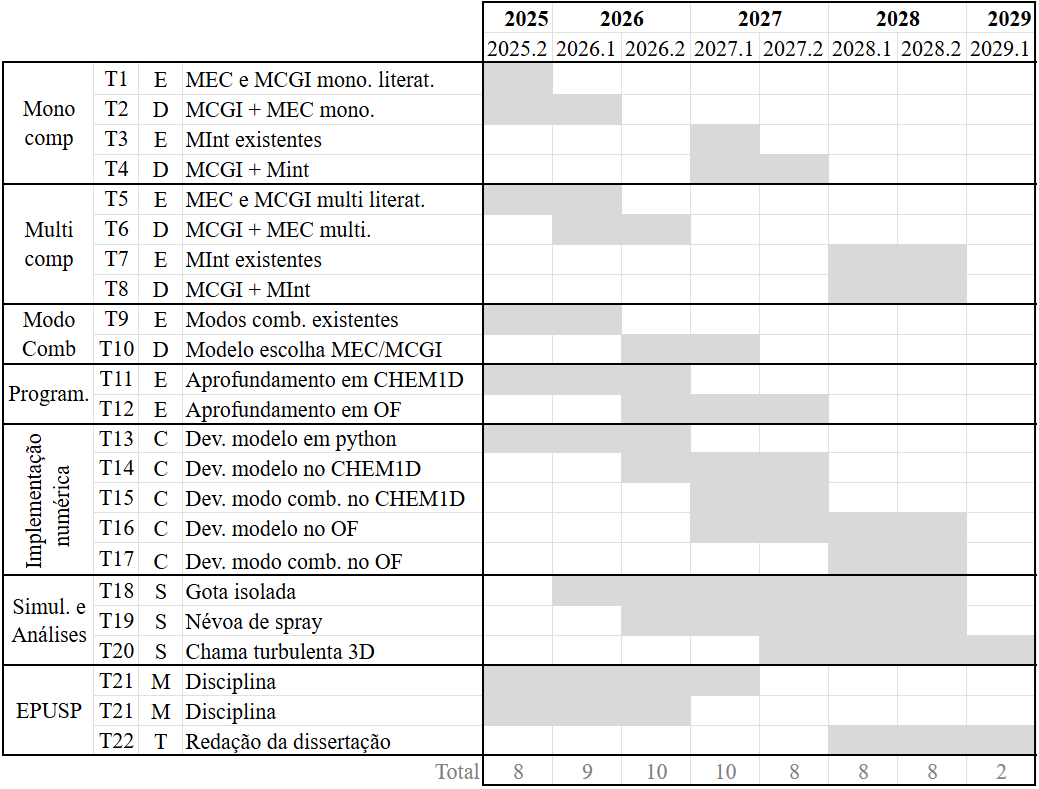
\includegraphics[width=0.9\textwidth]{30_images/cronograma-3.png}
    \label{fig:cronograma}
\end{figure}

O cronograma de excecução para essas tarefas ao longo do Doutorado pode ser encontrado na Figura \ref{fig:cronograma}.
As tarefas para essa proposta são expostas a seguir.

Considerando inicialmente gotas monocomponentes, incia-se com o estudo aprofundado sobre MEC e MCGI monocomponentes pré-existentes na literatura (\textbf{T1}), que dará base para o desenvolvimento de modelo integral de combustão de gota isolada monocomponente com modelo detalhado de evaporação (\textbf{T2}).
O estudo aprofundado de modelos pre-existentes para a modelagem analítica de \yellow{efeitos dos fenômenos HMT no} interior de gota é tarefa (\textbf{T3}), seguida pela avaliação da viabilidade de acoplamento de modelos monocomponente de combustão de gota isolada com discretização no interior da gota (\textbf{T4}).
A mesma sequencia de tarefas procede para gotas multicomponentes, originando as tarefas (\textbf{T5}), (\textbf{T6}), (\textbf{T7}) e (\textbf{T8}). 

Ainda no contexto de estudo e desenvolvimento analítico, encontra-se o estudo aprofundado de modelos de modo de combustão de sprays (\textbf{T9}) e a escolha dentre  ou desenvolvimento de um modelo analítico para determinar se a gota utiliza um MEC ou MCGI (\textbf{T10}).

Antes de iniciar as simulações, estão as tarefas referentes ao estudo aprofundado de dos softwares e linguagens de programação: CHEM1D e Fortran(\textbf{T11}), OpenFOAM e C++ 
(\textbf{T12}).

A implementação dos MEC e MCGIs desenvolvidos na linguagem Python pertence à tarefa  (\textbf{T13}),  CHEM1D à tarefa (\textbf{T14}) e no software OpenFOAM à tarefa (\textbf{T16}).
As tarefas (\textbf{T15}) e (\textbf{T17}) referem-se à implementação do algorítmo do modelo de modo de combustão, que fará a escolha entre MEC e MCGI, nos softwares CHEM1D e OpenFOAM respectivamente.

As simulações de evolução temporal de gota isolada em Python usando os MECs e MCGIs estão representadas pela tarefa (\textbf{T18}). 
A tarefa (\textbf{T19}) representa as simulações de chama combustão laminar em névoa quiescente de spray no CHEM1D, usando os modelos novos.
Já a tarefa (\textbf{T20}) refere-se às simulações de chama multidimensional turbulenta no OpenFOAM nas grandes escalas, usando FGM, ATG, e os modelos novos.
Essas tarefas de simulação incluem o pré-processamento, o tempo de simulação e a análise dos resultados (pós-processamento).
As ferramentas utilizadas para a análise dos resultados em cada uma das atividades de simulação são discutidas na Seção \ref{sec:resultados}.

O Programa de Pós-Graduacao em Engenharia Mecânica (PPGEM) da EPUSP exige que 9 disciplinas sejam cursadas para doutorado direto.
Elas são representadas pelas tarefas (\textbf{T20}) e (\textbf{T21}).
Algumas disciplinas se destacam devido a sua relevância para o tópico deste projeto \yellow{e foram selecionadas}: Fundamentos de Combustão I (PME5228), Fundamentos de Escoamentos Turbulentos Reativos  (PME5411), Sistemas Particulados (PQI5848), Termodinâmica Avançada I (PME5014), Introdução à Mecânica dos Meios Contínuos (PME5011) e Modelagem de Turbulência para CFD (PME5418).
Demais disciplinas serao definidas ao longo do desenvolvimento deste trabalho.

Por fim, a redação da dissertação é representada pela tarefa (\textbf{T22}).


% \begin{itemize}
%     \item[\textbf{T1}] Estudo aprofundado sobre MEC e MCGI monocomponentes pré-existentes na literatura.% Sobre o MEC, estão incluidos o estudo da derivação dos modelos de Abramzon-Sirignano \cite{Sirignano1989}, a formulação de Miller \cite{MillerR1998}, \todo{...}, No que tange a MCGIs, revisitar o modelo de Godsave-Spalding \cite{Law1978,HenningsJ2024MT}, estudar o artigo do Fachini \cite{FachiniF1999}, suas referências e citações, \todo{...} 
%     \item[\textbf{T2}] Modelagem analítica de combustão de gota isolada monocomponente com modelo detalhado de evaporação. % Essa tarefa baseia-se na incorporação do modelo de Abramzon-Sirignano \cite{Sirignano1989} ou da formulação de Miller \cite{MillerR1998} no modelo de Godsave-Spalding \cite{Law1978}. %Como todos os modelos citados baseiam-se em soluções analíticas, é visto como provável que 
%     \item[\textbf{T3}] Estudo de modelos pre-existentes para a modelagem  analítica de discretização do interior de gota monocomponente.% São exemplos de literatura relevante para essa tarefa \source{}.
%     \item[\textbf{T4}] Avaliação da viabilidade de acoplamento de modelos monocomponente de combustão de gota isolada com discretização no interior da gota.% Como os modelos de discretização de interior de gota podem envolver soluções numéricas, se será possível desenvolver uma solução analítica para esse problema. Uma solução acoplada numérica-analítica, interna e externamente gota, respectivamente, precisa ser robusta e computacionalmente eficiente para servir em aplicações CFD. 

%     \item[\textbf{T5}] Estudo de modelos MEC e MCGI multicomponente pre-existentes na literatura.% Exemplos de trabalhos relevantes de MEC multicomponente incluem \source{}.
%     \item[\textbf{T6}] Modelagem analítica de combustão de gota isolada multicomponente com modelo avançado de evaporação. % Essa tarefa baseia-se na incorporação dos modelos de Sacomano \cite{SacomanoF2022IJHMT} ou de Wang \source{WangC2012} no modelo de Godsave-Spalding \cite{Law1978}.
%     \item[\textbf{T7}] Estudo de modelos pre-existentes para a modelagem analítica de discretização do interior de gota multicomponente.% São exemplos de literatura relevante para essa tarefa \source{}
%     \item[\textbf{T8}] Avaliação da viabilidade de acoplamento de modelos multicomponente de combustão de gota isolada com discretização no interior da gota. 
    
%     \item[\textbf{T9}] Estudo de modelos de determinação de modos de combustão de gotas de spray, focando no modo de combustão isolada.% São exemplos de literatura relevante para essa tarefa \cite{AggarwalS2014}, \source{}
%     \item[\textbf{T10}] Desenvolvimento de modelo analítico para escolha entre MEC e MCGI, baseado na pesquisa do item anterior.
    
%     \item[\textbf{T11}] Approfundamento em CHEM1D e em Fortran para programação no CHEM1D.
%     \item[\textbf{T12}] Aprofundamento em OpenFOAM e em C++ para programação no OpenFOAM.
    
%     \item[\textbf{T13}] Implementação do modelo MEC/MCGI em Python.% para o T18.
%     \item[\textbf{T14}] Implementação do modelo MEC/MCGI no CHEM1D.% para o T19.
%     \item[\textbf{T15}] Implementação do modelo de modo de combustão no CHEM1D.
%     \item[\textbf{T16}] Implementação do modelo MEC/MCGI no OpenFOAM.% para o T20.
%     \item[\textbf{T17}] Implementação do modelo de modo de combustão no OF.
    
%     \item[\textbf{T18}] Simulação da evolução temporal 0D de gota isolada em Python.           %, após T15.
%     \item[\textbf{T19}] Simulação de combustão laminar de névoa quiescente de spray no CHEM1D. %, após T16.
%     \item[\textbf{T20}] Simulação de chama turbulenta 3D nas grandes escalas com FGM e ATF.    %, após T17.
    
%     \item[\textbf{T21}] Disciplinas de pós-graduação.% No programa de Doutorado Direto do PPGEM na POLI-USP, é necessário cursar 9 Disciplinas, cada valendo 8 créditos. Como não é recomendado cursar mais de duas disciplinas por oferencimento, o qual é quadrimestral, as disciplinas serão cursadas ao longo de 5 quadrimestres, aproximadamente 2 anos. Algumas das disciplinas a serem cursadas já foram escolhidas e estão dispostas na Seção \ref{sec:disciplinas}.
%     \item[\textbf{T22}] Redação da dissertação.% Estimou-se iniciar a escrita da dissertação nos últimos três semestres.
% \end{itemize}

% \subsection{Disciplinas a serem cursadas} \label{sec:disciplinas}


         % Plano de Trabalho e Cronograma de Excecução
% !TEX root = ../Proposta.tex

\section{Forma de Análise dos Resultados} \label{sec:resultados}

Diferentes procedimentos serão adotados para a análise dos resultados obtidos em cada etapa de trabalho apresentada na Seção \ref{sec:metod}.
Considerando apenas os resultados numéricos, i.e. das de simulações, os primeiros resultados serão obtidos após o teste do modelo isolado em ambiente Python. 

A simulação da evolução temporal de um modelo de gota, MEC ou MCGI, e a análise desses resultados é uma área que o autor da proposta já tem experiência \cite{HenningsJ2024MT}. 
Nessa análise, são relevantes parâmetros como o tempo de vida gota, a dependência dos resultados ds condições iniciais da gota e do ambiente e a dependência dos submodelos utilizados, como o de pressão de vapor ou de fração molar de vapor.
% Além disso, será util também a experiência do autor com análise paramétrica de sistemas fluidodinâmicos e computação científica \source{Meus 3 artigos}.

No contexto de avaliação isolada de MECs e MCGIs, é de extrema relevância a comparação tanto com resultados experimentais quanto como \yellow{modelos resolvidos}.
Para MECs, considera-se, por exemplo, os trabalhos experimentais \cite{BiroukM2006,PatelU2019,KayaEyiceD2024,ArabkhalajA2024,MaquaC2008}, focados principalmente na influência da turbulência na evaporação.
Para MCGIs, considera-se os trabalhos experimentais na escala da gota \cite{ChoS1990SCI,CandelS1999,ChenG1996CF,Xu2002,BiroukM2000,CuociA2005,SetyawanH2015} e os trabalhos que \yellow{resolvem} o modelo da gota \cite{Stauch2006,CuociA2005,ChoS1990SCI,KazakovA2003CF,MarcheseA1996CF,WangW2024}.

Já nas simulações no CHEM1D, a análise dos resultados se dará baseada na experiência do grupo de pesquisa, assim como na comparação com MECs já desenvolvidos pelo grupo e testados nesse ambiente \cite{SacomanoF2018CTM,SacomanoF2019IJHMT,SacomanoF2021Fluids,SacomanoF2024CF,SacomanoF2025CF}.
Nessas simulações, são relevantes novamente a influência das condições iniciais e ambientais na frente de chama, em particular na velocidade de chama laminar.

Nas simulações multidimensionais, também será valiosa a experiência e os resultados anteriores do grupo de pesquisa \cite{SacomanoF2017CF,SacomanoF2020CF}.
Nessas simulações, é relevante estudar a influência do modo de combustão de gota isolada na estrutura da chama, como proposto nos objetivos do trabalho.
% Para validação dos resultados, são relevantes os trabalhos de larga escala em queimadores experimentais pelo mundo  (\emph{c.f.} \source{MasriA2021} para exemplos e referências)

% Comparação com experimentais \source{} e casos resolveram a gota \source{}.

% Experimentos evaporação:  Spray Combustion, Seção 4.1
% Experimentos comvustão de gota isolada: Spray Combustion, Seção 4.2

% Simulação resolvida evap: Spray Combustion, Seção 5.1
% Simulação resolvida gota isolada: Spray Combustion, Seção 5.2    % Resultados Esperados // Forma de análise dos resultados

\newpage
\bibliographystyle{abntex2-alf}
\bibliography{bibliography,bibliography2}


\end{document}
